\chapter{Resultados e Discussões}
\label{cap:resultados}
Este capítulo apresenta os resultados obtidos com a execução dos testes de carga descritos no \autoref{cap:estudo_caso1}. Além disso, há uma discussão geral sobre o processo de desenvolvimento do caso de uso com a utilização da \acrfull{ams} e \acrfull{ddd}.

\section{Resultados}
Essa seção apresenta uma análise gráfica dos resultados obtidos com a execução dos testes de carga. Os gráficos foram gerados pelo \english{AWS CloudWatch} a partir das métricas coletadas dos serviços de computação e banco de dados da \english{Amazon Web Services} durante a execução dos testes. Os dados apresentados apresentam a média dos serviços.

\subsection{Utilização da CPU}
Na \autoref{fig:cpu-utilization} é possível observar a utilização da CPU durante a execução dos testes de carga. Durante toda a simulação, a utilização de CPU se manteve em torno de 35\%, um valor considerado baixo. Isso indica que o sistema é capaz de suportar um número maior de requisições sem que haja um aumento significativo na utilização de CPU. Esse valor também está abaixo do alvo de 70\% estabelecido anteriormente. 

\begin{figure}[H]
    \centering
    \caption{Utilização da CPU}
    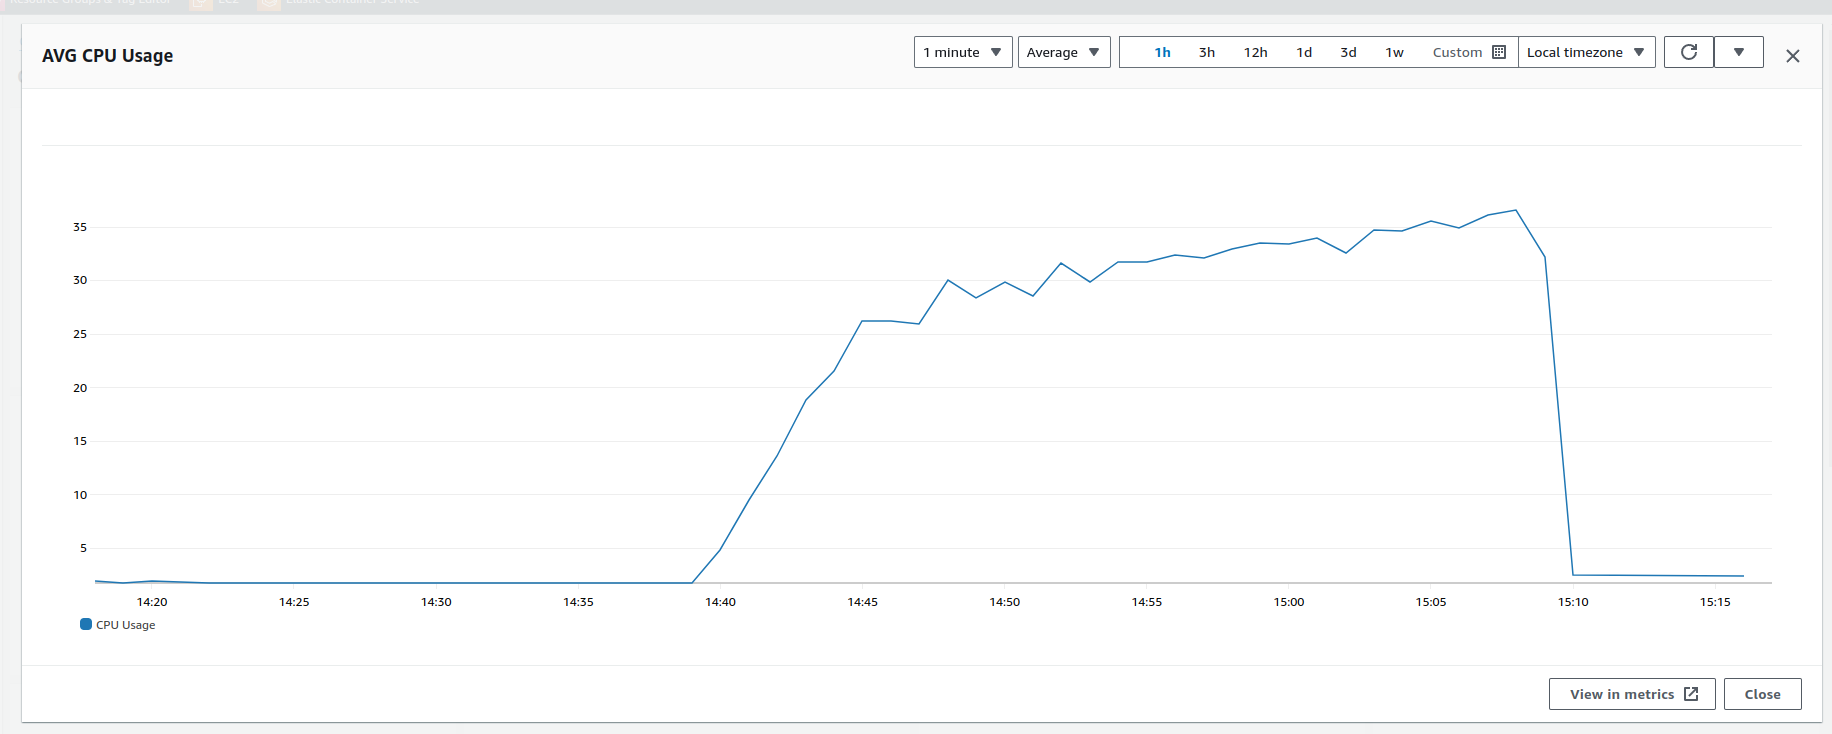
\includegraphics[width=0.8\textwidth]{media/cpu-usage.png}
    \fonte{o autor}
    \label{fig:cpu-utilization}
\end{figure}

\subsection{Utilização da Memória RAM}
Na \autoref{fig:memory-utilization} é possível observar a utilização da memória RAM durante a execução dos testes de carga. Houve um uso muito baixo de memória, com uma média em torno de 7\%. Isso indica que o sistema como um todo é \english{CPU-bound}, termo utilizado para descrever sistemas que são limitados pela CPU e não pela memória. Essa métrica também ficou abaixo do alvo.

\begin{figure}[H]
    \centering
    \caption{Utilização da Memória RAM}
    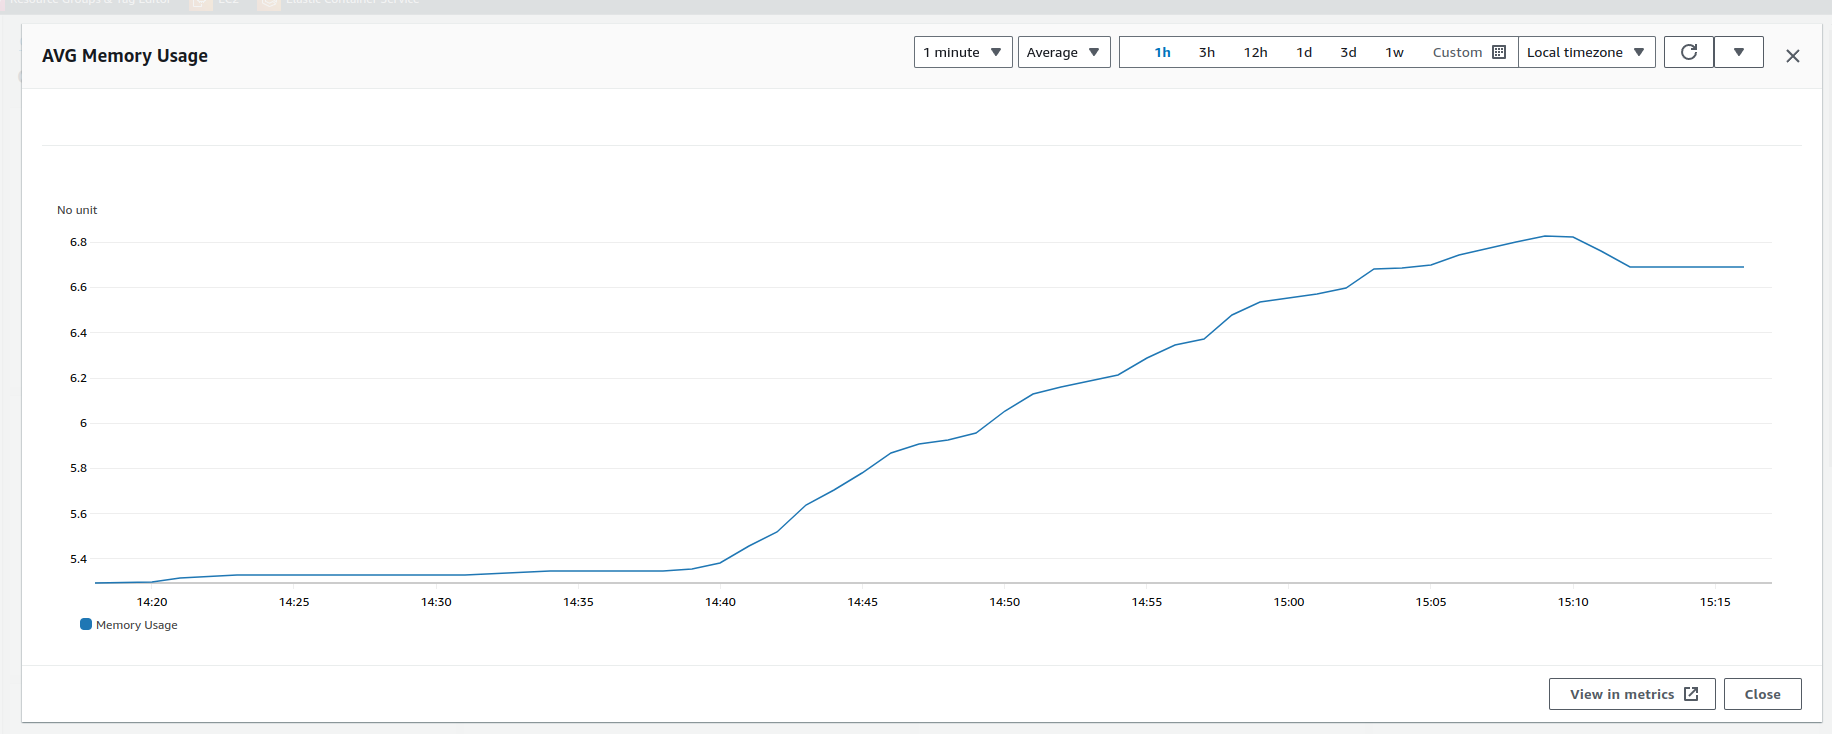
\includegraphics[width=0.8\textwidth]{media/memory-usage.png}
    \fonte{o autor}
    \label{fig:memory-utilization}
\end{figure}

\subsection{Tempo de Resposta}
Na \autoref{fig:response-time} é possível observar o tempo de resposta das requisições durante a simulação. Utilizando como base o P90, o tempo de resposta se manteve em torno de 1 segundo, um valor considerado aceitável. Esse valor também está abaixo do alvo de 2 segundos estabelecido anteriormente.

\begin{figure}[H]
    \centering
    \caption{Tempo de Resposta}
    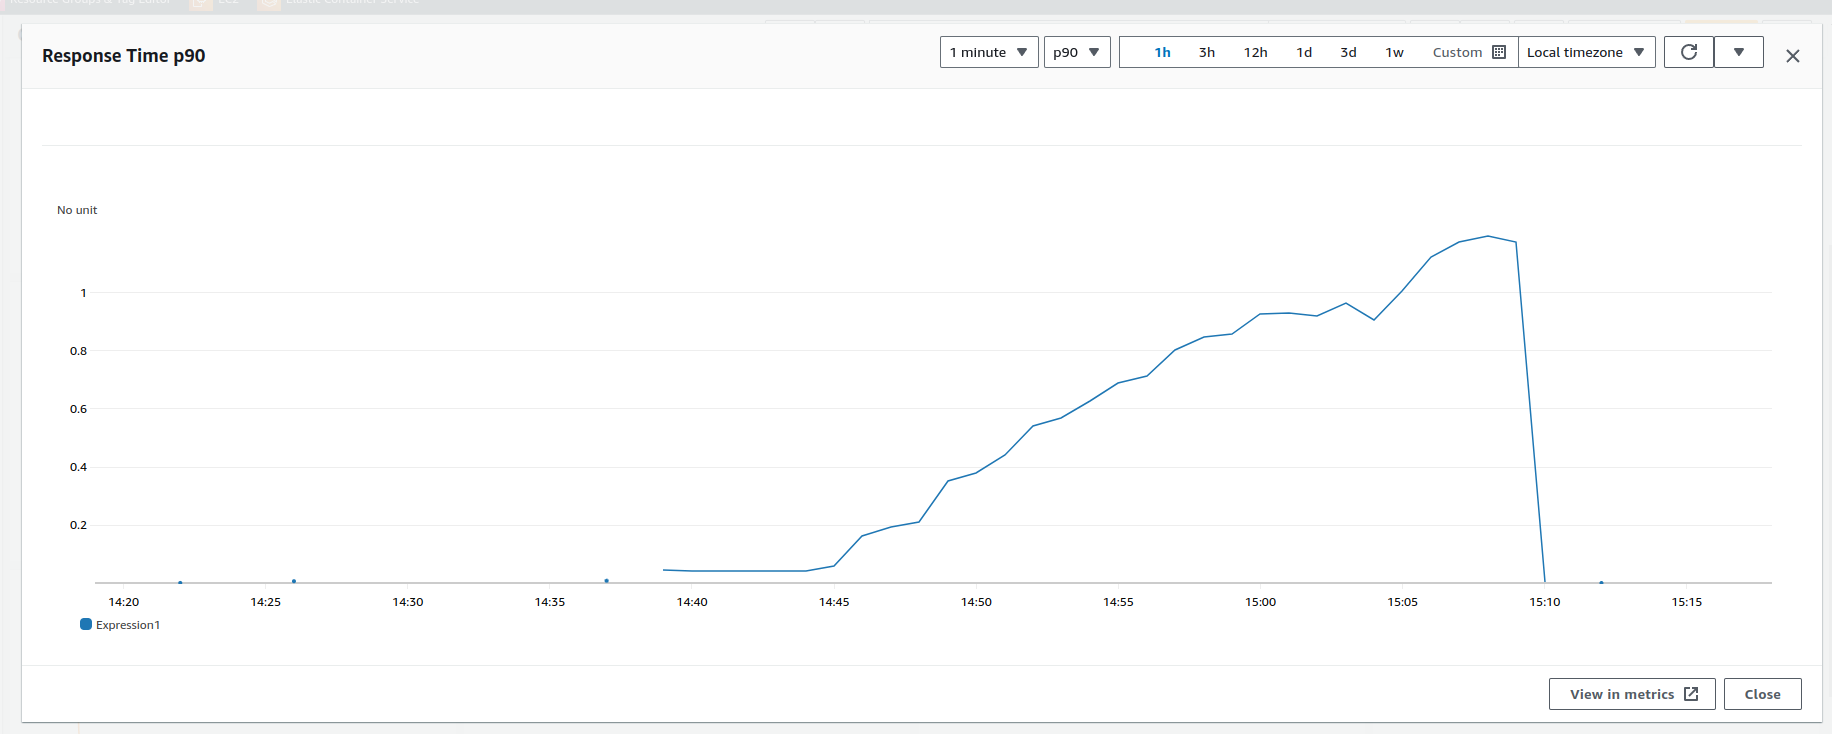
\includegraphics[width=0.8\textwidth]{media/response-time.png}
    \fonte{o autor}
    \label{fig:response-time}
\end{figure}

\subsection{Porcentagem de erros}
Na \autoref{fig:error-rate} é possível observar a porcentagem de erros durante a execução dos testes de carga. Durante toda a simulação, a porcentagem de erros se manteve em 0.2\% (média), indicando que o sistema é capaz de suportar um grande número de requisições sem impactar os usuários. Esse valor também está abaixo do alvo de 1\% estabelecido anteriormente.

\begin{figure}[H]
    \centering
    \caption{Porcentagem de Erros}
    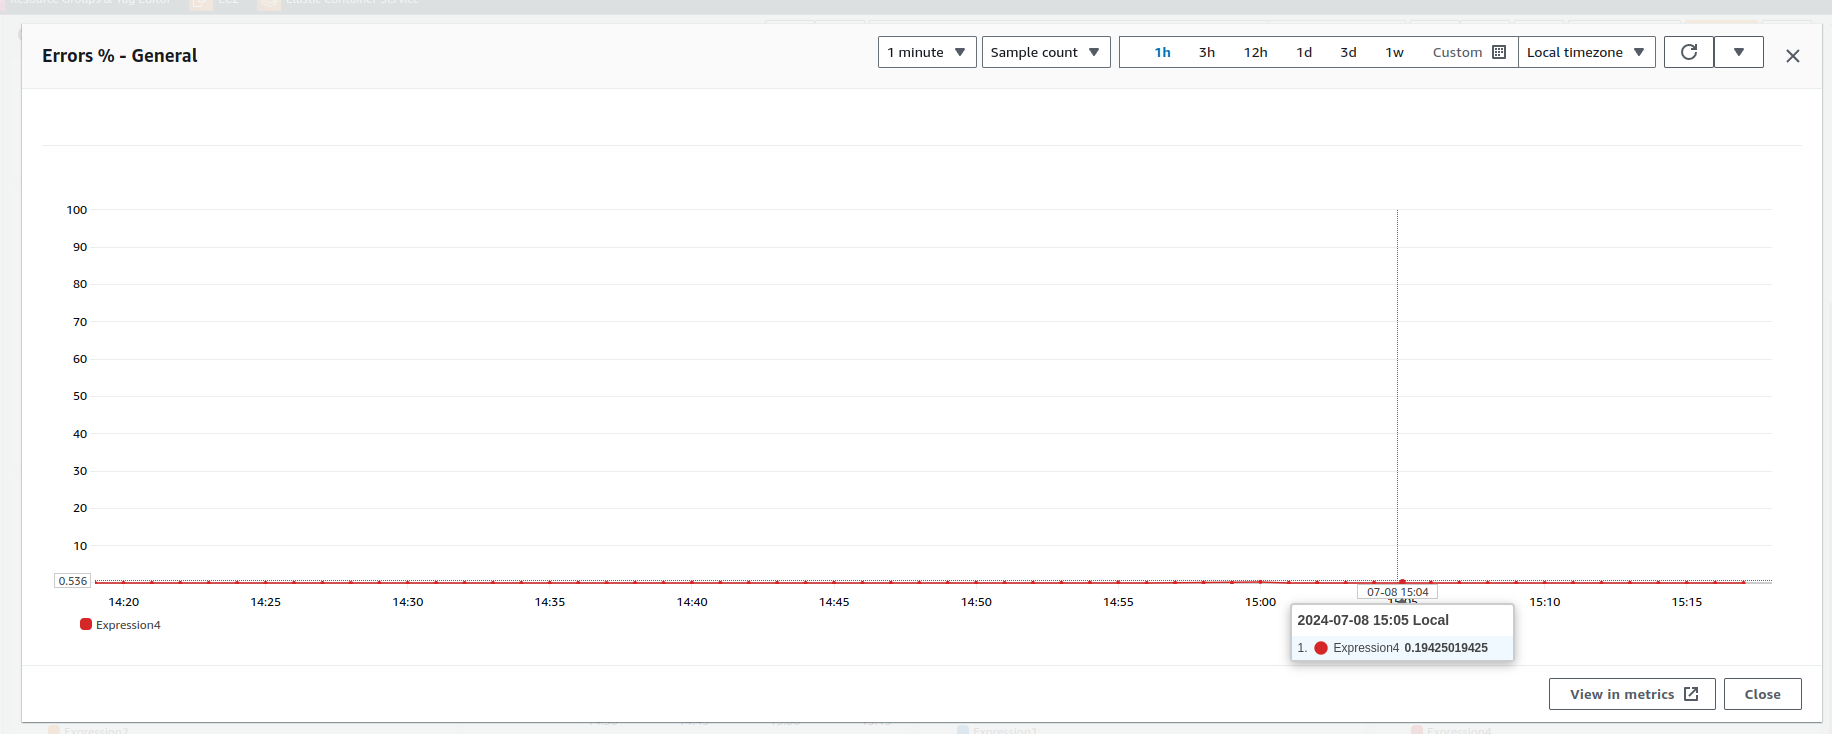
\includegraphics[width=0.8\textwidth]{media/errors.png}
    \fonte{o autor}
    \label{fig:error-rate}
\end{figure}

\section{Trabalhos Futuros}
Como trabalhos futuros, é possível destacar a construção de novos estudos de caso com a utilização de \acrshort{ddd} e \acrshort{ams} em outros contextos complexos como, por exemplo, sistemas financeiros, sistemas de logísticas e sistemas de saúde. Além disso, um trabalho futuro interessante seria a comparação de entre dois sistemas de domínios iguais, um desenvolvido com as técnicas apresentadas nesse trabalho e um outro somente com \acrshort{ddd} ou \acrshort{ams}. Assim, seria possível quantificar os benefícios e desvantagens da utilização dessas tecnologias em conjunto.

\section{Discussões}
Essa seção apresenta uma discussão geral sobre o processo de desenvolvimento do caso de uso com a utilização da \acrfull{ams} e \acrfull{ddd}. A utilização dessas tecnologias trouxe diversos desafios e benefícios ao desenvolvimento do sistema.

A separação de serviços em microsserviços permitiu que cada parte do sistema fosse desenvolvida de forma independente, facilitando a manutenção e evolução do sistema. Além disso, a utilização de \acrfull{ddd} permitiu que o domínio do negócio fosse modelado de forma mais clara e eficiente, facilitando o entendimento do sistema como um todo.

Da mesma forma, como cada microsserviço tem um foco específico, se torna mais fácil o entendimento de como cada parte do sistema funciona. Isso também facilita a escalabilidade do sistema, uma vez que é possível escalar apenas os serviços que estão sobrecarregados.

A utilização de \acrfull{ams} e \acrfull{ddd} trouxe diversos desafios ao desenvolvimento do sistema. O maior deles foi a necessidade de um maior esforço de \english{design upfront} para garantir a correta separação de serviços e a definição do domínio do negócio. Isso se deve ao fato de que a separação de serviços em microsserviços e a utilização de \acrfull{ddd} requerem um maior entendimento do negócio e da arquitetura do sistema.

Além disso, a complexidade aumentada para criação e execução de testes também foi um desafio. Como cada microsserviço é um sistema independente, é necessário criar testes para cada parte do sistema, o que aumenta a complexidade dos testes.

Outro desafio foi o maior custo computacional para executar o sistema localmente. Como cada microsserviço é uma aplicação independente, possui seu próprio processo em nível de sistema operacional, o que aumenta o custo computacional para executar o sistema localmente. Assim, os desenvolvedores precisam de máquinas mais potentes.

Por fim, a maior complexidade de deploy também foi um desafio. É necessário criar mais serviços, configurar máquinas virtuais, \english{load balancers} e banco de dados. Além disso, é importante configurar corretamente a rede para garantir a comunicação entre os serviços. Inicialmente, se tem um custo maior para manter o sistema em produção. Porém, com o crescimento do tráfego, a escalabilidade do sistema se torna mais fácil.